% !TEX root = Projektstudie.tex
% Ausblick

\section{Ausblick}
\label{sec:Ausblick}
% - NOT-AUS Schalter
% - Arduino-Shield
% - Deckenkamera
% - Hindernissen ausweichen (Dijkstra?)
% - Steuerung übers Netzwerk / W-Lan: Python Flask Server + Raspberry

\subsection{Schutzbeschaltung}
\label{sec:Schutzbeschaltung}
%NOT-AUS
Um einen sicheren Betrieb des Roboters sicher zu stellen, muss ein NOT-AUS-Schalter nachgerüstet werden. Dieser muss in der Lage sein jede Bewegung des Roboters zu beenden.
\begin{itemize}
\item{Im Netzbetrieb an einer Verlängerungsleitung muss der NOT-AUS-Schalter den Roboter von der Netzspannung trennen.}
\item{Im Akkubetrieb muss der NOT-AUS-Schalter beide Pole vom Akku abschalten.}
\end{itemize}
In beiden Fällen muss der 

\subsection{Arduino-Shield}
\label{sec:Arduino-Shield}
Da der Speicher des verwendeten Arduino UNO bereits zu $78\%$ ausgelastet ist, wird in Ergänzung zum Sparkfun CAN-Shield ein eigenes CAN-Shield für den leistungsfähigeren Arduino MEGA 2560 entwickelt.
 
Durch geschickte Wahl der Anschlusspins wird die optional angedachte Verwendung des Arduino-Ethernet-Shield ermöglicht. Hierzu werden der Ethernet-Shield und der entwickelte CAN-Bus-Shield auf den Arduino gestapelt aufgesteckt. Neben CAN-Bus-Stecker und –Buchse mit erforderlicher Elektronikbeschaltung besitzt das Layout Anschlussklemmen für $5V$ Spannungsversorgung und $I^{2}C$-Bus.

Das Platinenlayout ist als Double Layer Platine ausgeführt. In der folgenden Abbildung
sind die Abmessungen der Bauteile  in Grau, Lötpads in Grün, die Top Kupferflächen und Leiterbahnen in Rot und die Kupferflächen  und Leiterbahnen auf der Bottom Seite in Blau dargestellt.

\begin{figure}[H]
\centering
 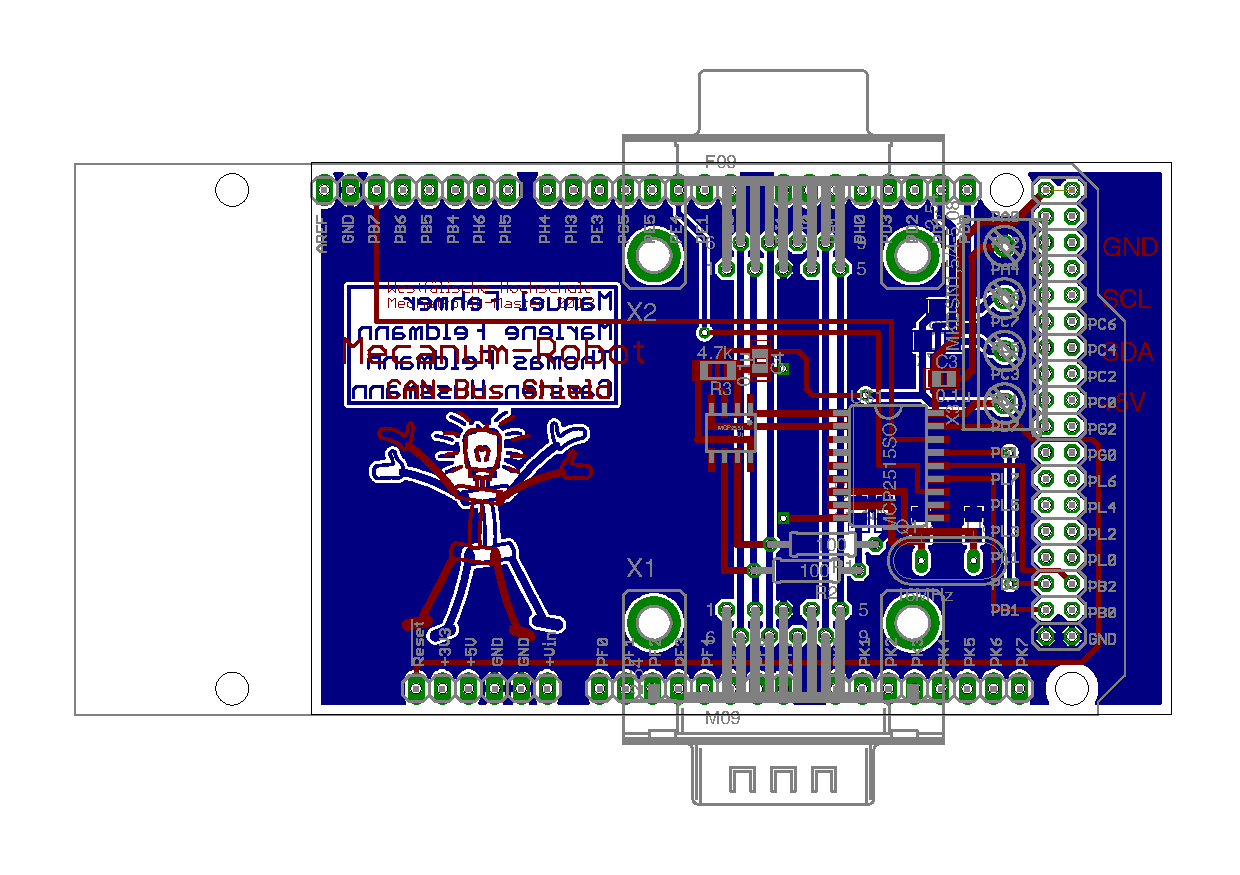
\includegraphics[width=0.8\textwidth]{Abbildungen/CAN-Shield-Layout} 
\caption[CAN-Shield-Layout]{CAN-Shield-Layout}
\label{fig:CAN-Shield-Layout}
\end{figure}

\begin{figure}[H]
\centering
 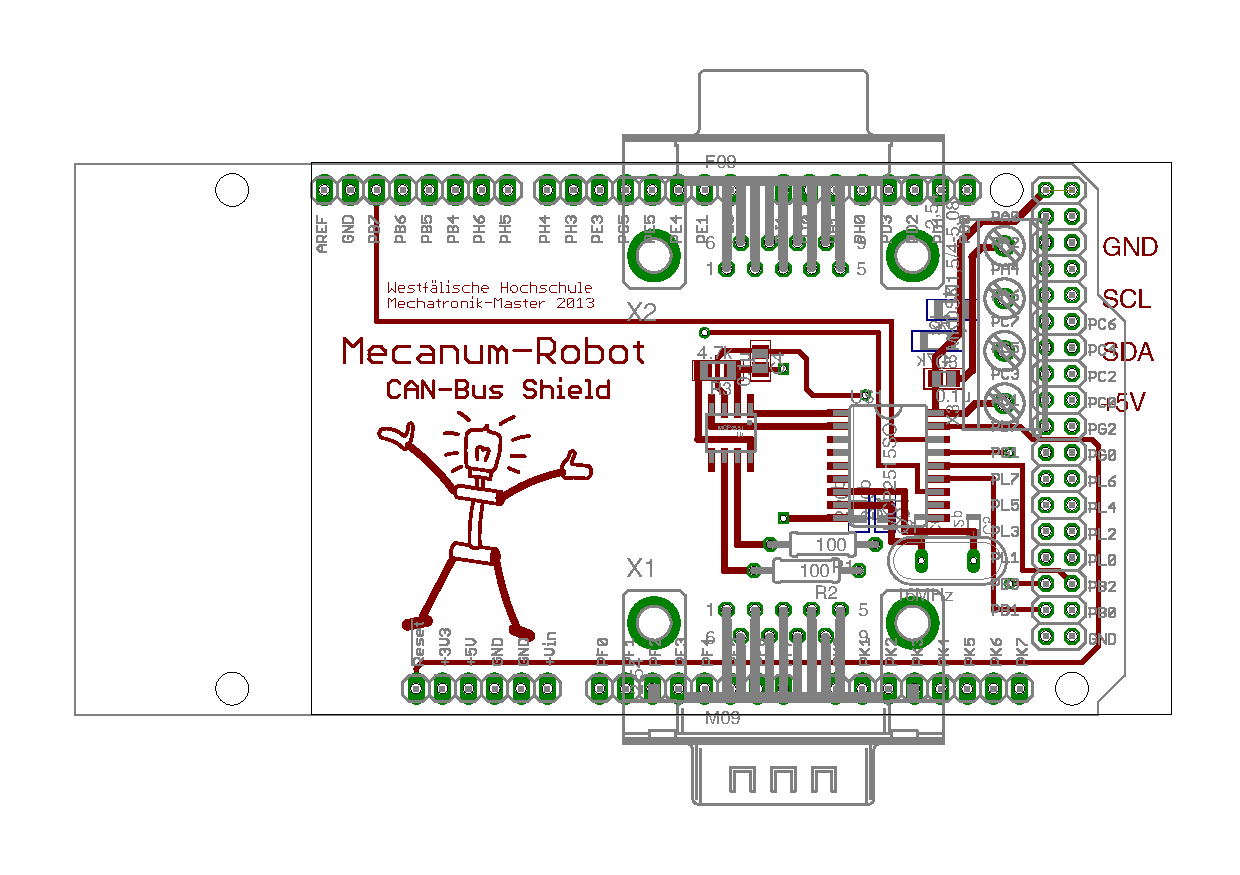
\includegraphics[width=0.8\textwidth]{Abbildungen/CAN-Shield-Layout-Top} 
\caption[CAN-Shield-Top-Layer]{CAN-Shield-Top-Layer}
\label{fig:CAN-Shield-Layout-Top}
\end{figure}

\begin{figure}[H]
\centering
 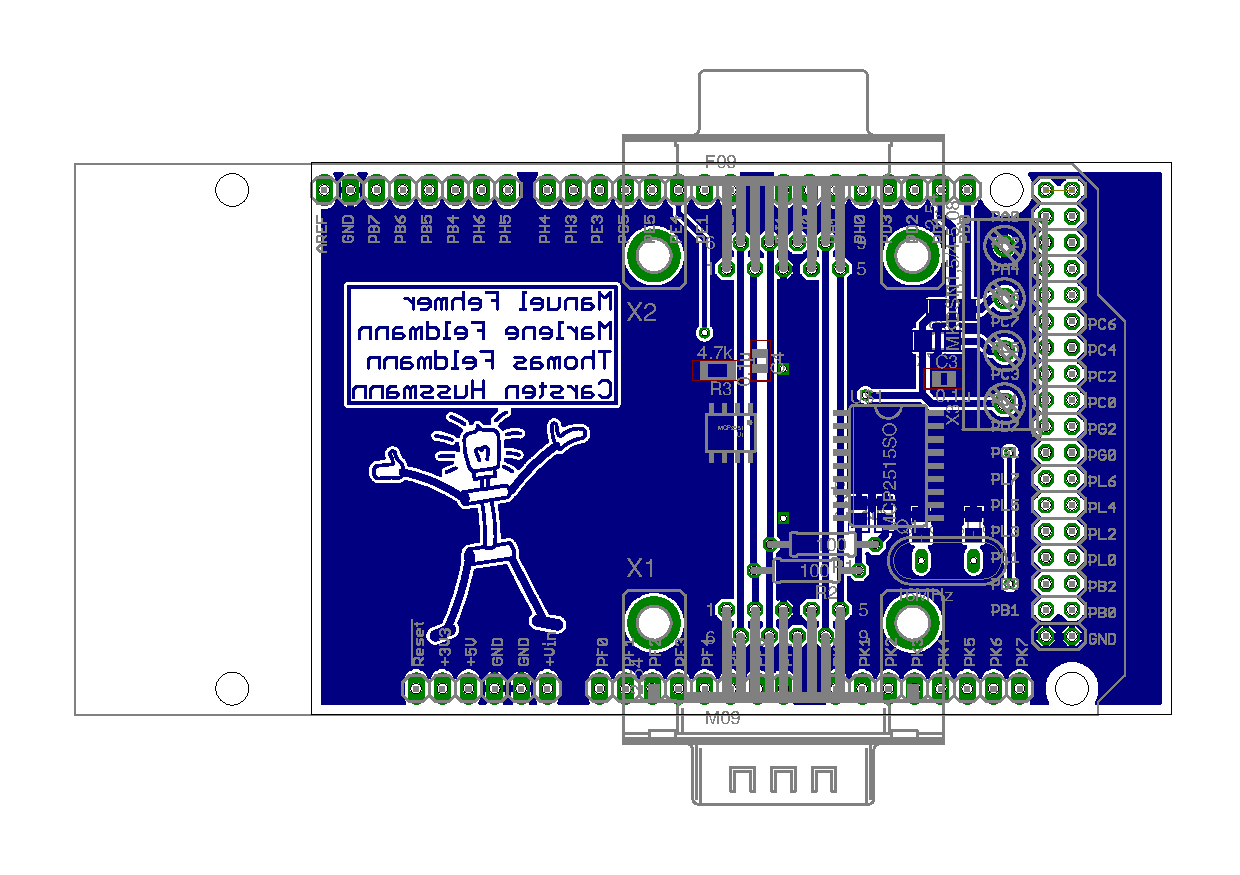
\includegraphics[width=0.8\textwidth]{Abbildungen/CAN-Shield-Layout-Bottom} 
\caption[CAN-Shield-Bottom-Layer]{CAN-Shield-Bottom-Layer}
\label{fig:CAN-Shield-Layout-Bottom}
\end{figure}
